%
% File acl2015.tex
%
% Contact: car@ir.hit.edu.cn, gdzhou@suda.edu.cn
%%
%% Based on the style files for ACL-2014, which were, in turn,
%% Based on the style files for ACL-2013, which were, in turn,
%% Based on the style files for ACL-2012, which were, in turn,
%% based on the style files for ACL-2011, which were, in turn,
%% based on the style files for ACL-2010, which were, in turn,
%% based on the style files for ACL-IJCNLP-2009, which were, in turn,
%% based on the style files for EACL-2009 and IJCNLP-2008...

%% Based on the style files for EACL 2006 by
%%e.agirre@ehu.es or Sergi.Balari@uab.es
%% and that of ACL 08 by Joakim Nivre and Noah Smith

\documentclass[11pt]{article}
\usepackage[utf8]{inputenc}
\usepackage[T1]{fontenc}
\usepackage{acl2015}
\usepackage[backend=biber,
            style=authoryear-icomp,
            doi=false,
            isbn=false,
            url=false,
            maxcitenames=1]{biblatex}
\usepackage{times}
\usepackage{url}
\usepackage{latexsym}% -*- program: Value -*-
\usepackage{graphicx}
\usepackage[colorlinks=false, pdfborder={0 0 0}]{hyperref}
\usepackage{cleveref}
\usepackage{booktabs}
\usepackage{adjustbox}
\addbibresource{bibliography.bib}
%\setlength\titlebox{5cm}

% You can expand the titlebox if you need extra space
% to show all the authors. Please do not make the titlebox
% smaller than 5cm (the original size); we will check this
% in the camera-ready version and ask you to change it back.


\title{POS driven Cross-Lingual Pronoun Prediction with Feed-Forward Neural Networks}

\author{Jimmy Callin \\
  Uppsala University \\
  {\tt jimmy.callin@gmail.com}}

\date{}

\begin{document}
\maketitle
\begin{abstract}
    In some languages, pronoun translation is a discourse driven task. We suggest a neural network based model using preceding nouns and determiners as features for suggesting antecedent. Our model scores on par with similar models while having a simpler architecture.
\end{abstract}


\section{Introduction}

When translating between languages, there are several discourse phenomena that are more difficult to translate than others.
For instance, the act of translating pronouns usually requires insight into what is the antecedent of said pronoun, since gender of noun phrases rarely translate well between languages.
While we have started to see a movement towards machine translation models that do not treat sentences in isolation, discourse oriented systems have yet to introduce performance improvements that would motivate ubiquotous usage.

In light of this, there have previously been attempts at treating pronoun translation as a classification task separate from machine translation.
In this fashion a pronoun translation module could potentially be treated as just another part of translation by discourse oriented machine translation systems, or as a post-processing step in systems where translations using larger contexts than sentence-level simply are not supported (such as Moses).
Also, in case of a successful pronoun prediction model, it could potentially lead to further insights into the nature of anaphora resolution.
DiscoMT 2015 introduces the shared task of cross-lingual pronoun prediction.

What is given are documents in a source language (English, in this case), a translation to a target language (French), as well as word alignments.
The word alignments are automatically produced by GIZA++.
What is missing are third-person pronouns in the target translation.
While English pronoun usage is relatively easy to infer from the immediate context, this is not the case in all languages.
When translating to French, for instance, the translator requires to keep the immediate antecedent in mind for determining the use of male (\emph{elle}) or female (\emph{elles}) third-person pronoun.
This is something you simply cannot infer from context alone.


\section{Data}

Several training resources were provided as a part of this task.
For training, transcribed TED talks are available.
Additionally, Europarl contains extracted proceedings from the European government.
A corpus of news text was included as well. Test data is a collection of transcribed TED talks, in total 12 documents containing 2093 sentences with a total of 1105 classification problems.
All of these resources are English-French parallell corpora with automatically generated word alignments.

\section{Method}

Inspired by the the neural network architecture set up in \cite{Hardmeier2013Latent}, we similarly propose a feed-forward neural network with a layer of word embeddings as well as an additional hidden layer for learning abstract .
The model is trained using stochastic gradient descent with mini-batches and L2 regularization.
Cross-entropy is used as a cost function.
Main difference lies in avoiding using antecedent features as gathered by an external anaphora resolution system.
Rather, to simplify the model we try to simply look at the four closest previous nouns and determiners in English, and use the corresponding aligned French nouns and articles in the model, as illustrated in \cref{fig:posexample}.
Wherever the alignments map to more than one word, only the furthermost left of the words in the phrase is used.

\begin{figure}[htbp]
    \centering
    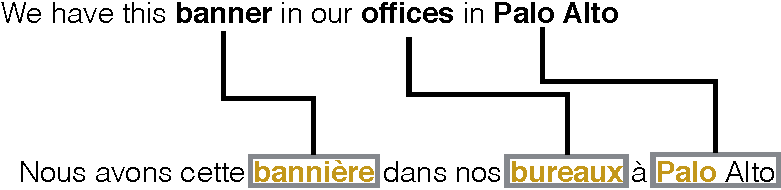
\includegraphics[width=0.5\textwidth]{figures/posexample.pdf}
    \caption{An English POS tagger is used to find nouns and articles in preceding utterances, while the word alignments determine which French words are to be used as features.}
    \label{fig:posexample}
\end{figure}


Additionally, we allow ourselves to look at the French context of the missing pronoun.
While this restricts the potential usage of our model as a part of the translation process, French usage should be a better indicator for some of the classes.
Especially \emph{ce}, which is highly dependent being precedent of \emph{est}.
See \cref{fig:contextexample} for an example.

Furthermore the dimensionality of the embeddings are increased from 20 to 50, since this was empirically shown to somewhat improve the scores on the development set, with a hidden layer size of 50.
To reduce training time and faster find convergence, we use $\tanh$ as activation function between the hidden layers, in contrast to the sigmoid function in the original paper (\cite{Lecun2012Efficient}).
To avoid overfitting, early stopping is introduced where the training stops if no improvements have been found within a number of iterations.
This usually results in a training time of 130 epochs, when run on TED data from IWSLT.

It uses a uniform random weight initialization according to \textcite{Glorot2010Understanding}, where they show that neural network models using $\tanh$ as activation function generally perform better with an initialization within the interval $uniform[-\frac{\sqrt{6}}{\sqrt{fan_{in}+fan_{out}}},\frac{\sqrt{6}}{\sqrt{fan_{in}+fan_{out}}}]$, where $fan_{in}$ and $fan_{out}$ are number of inputs and number of hidden units respectively.

The final architecture as shown in \cref{fig:nnarchitecture} was implemented in Theano \cite{Bergstra2010Theano}, and is publicly available on Github\footnote{\url{http://github.com/jimmycallin/whatelles}}.
The final parameters used are a 4+4 context window for English and French, with 3 preceding nouns and articles each.

\begin{figure*}[htbp]
    \centering
    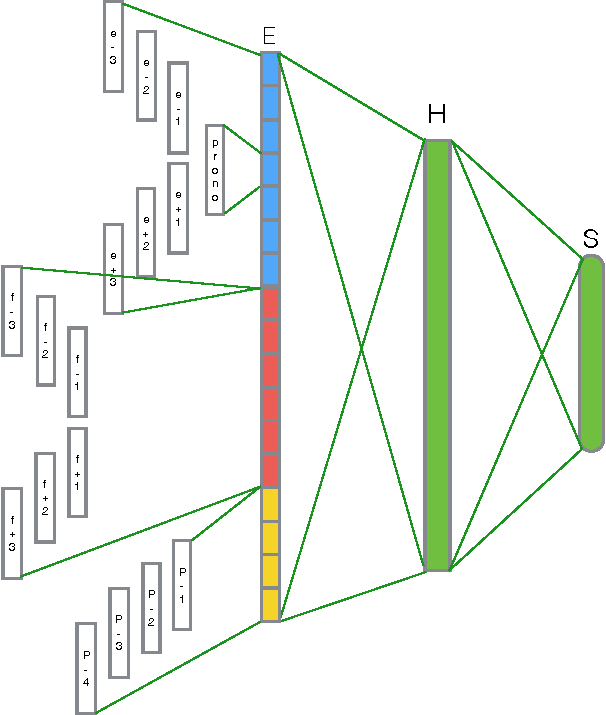
\includegraphics[width=0.4\textwidth]{figures/nnarchitecture.pdf}
    \caption{Neural network architecture. Blue embeddings (E) signifies source context, red target context, and yellow the preceding POS tags. The shown number of features is not equivalent with what is used in the final model.}
    \label{fig:nnarchitecture}
\end{figure*}

\begin{figure}[htbp]
    \centering
    
\includegraphics[width=0.5\textwidth]{figures/contextexample.pdf}
    \caption{Example of context used in the classification model, color coded according to their position in the neural network as illustrated in \cref{fig:nnarchitecture}.}
    \label{fig:contextexample}
\end{figure}

\section{Results}

The results are presented in \cref{tbl:resultscores} with a confusion matrix in \cref{tbl:confmatrix}.
Best performing classes are \emph{ce}, \emph{ils}, and \emph{other}, while the less commonly occurring classes \emph{elle} and \emph{elles} have precision comparable to other classes.
Their recall, though, is significantly worse. The overall macro F1 score ends up being 55.3\%.

\begin{table}[t]
\center
    \begin{tabular}{llll}
          & Precision & Recall  & F1      \\ \midrule
    ce    & 0.8291   & 0.8967 & 0.8616 \\
    cela  & 0.7143   & 0.6202 & 0.6639 \\
    elle  & 0.5000   & 0.2651 & 0.3465 \\
    elles & 0.6296   & 0.3333 & 0.4359 \\
    il    & 0.5161   & 0.6154 & 0.5614 \\
    ils   & 0.7487   & 0.9312 & 0.8301 \\
    other & 0.8450   & 0.8579 & 0.8514 \\
    \midrule
    Macro & 0.5816 & 0.5495 & 0.5530 \\
    Micro & 0.7213 & 0.7213 & 0.7213 \\
    \hline
    \end{tabular}
    \caption{Precision, recall, and F1-score for all classes. Micro score is the overall classification score, while macro is the average over each class. The latter scoring method is used for increasing the importance of classes with fewer instances.}
    \label{tbl:resultscores}
\end{table}

\begin{table}[t]
    \center
    \scalebox{0.8}{
    \begin{tabular}{@{}rlllllll@{}}
          & ce  & cela & elle & elles & il  & ils & other      \\
    ce    & 165 & 3    & 0    & 1     & 8   & 1   & 6      \\
    cela  & 5   & 80   & 4    & 1     & 21  & 0   & 18     \\
    elle  & 7   & 10   & 22   & 2     & 22  & 2   & 18     \\
    elles & 0   & 0    & 0    & 18    & 0   & 31  & 3      \\
    il    & 11  & 7    & 9    & 0     & 64  & 1   & 12     \\
    ils   & 1   & 0    & 0    & 5     & 0   & 149 & 5      \\
    other & 10  & 12   & 9    & 1     & 9   & 15  & 338    \\
    \end{tabular}}
    \caption{Confusion matrix over class predicitons. Row signifies actual class according to gold standard, while column represents predicted class according to the classifier.}
    \label{tbl:confmatrix}
\end{table}

\section{Discussion}

Results indicate that the model performs on par with previously suggested models, while having a simpler architecture.
The classes of feminine gender does not perform as well, especially not recall-wise, although this was to be expected since the only real information from which to infer its antecedent is distance from the pronoun in focus.
It is apparent that the model have a bias towards making majority class predictions.
An additional hypothesis is that it is simply too little data to realistically create usable embeddings, except for in a few reoccurring circumstances.

The extra number of features as well as the increase in embedding dimensionality makes the training and prediction somewhat slower, but since the training still is done in less than an hour, and predicting the test data doesn't take more than a few seconds, it is still good enough for general usage.
Furthermore, the implementation is made in such a way that further performance increases are to be expected if you run it on CUDA compatible GPU with minor changes.

While three separate training data collections were available, in the end only transcribed TED talks were used, which is of the same domain as the test data.
To overcome the skew class distribution, attempts were made at oversampling the less frequent classes from Europarl, but unfortunately this only led to performance loss on the development set.
The model does not seem to generalize well from other types of training data such as Europarl or News text, despite Europarl being transcribed speech as well.
This is an obvious shortcoming of the model.

We tried several alterations in parameter settings for context window and POS tags, and there were no significant improvements found beyond the final parameter settings when run on the development set.
In future work, it would be interesting to look into whether source context actually contribute to the pronoun prediction at all.
The English context is indeed nice to have, since you cannot be entirely certain of the translation quality in the target language, but intuitively all necessary linguistic information should only be available in the target language.
If source language were to be used, each English word embedding could perhaps be pre-trained on a large number of translation examples hopefully learning the most probable cross-linguistic gender.
Gender aware French word embeddings would hypothetically increase the score as well, if not more.

\section{Conclusion}

In this work, we have been developing a cross-lingual pronoun prediction classifier based on a feed-forward neural network.
The model was heavily inspired by (\cite{Hardmeier2013Latent}), while trying to simplify the architecture by simply using preceding nouns and determiners for coreference resolution rather than using features from an anaphora extractor such as BART, as set up in the original paper, since these usually includes large performance overhead.

We find out that the model indeed perform on par with similar models, while being easier to train.
There are some expected drops in performance for the less common classes heavily dependent on finding the correct anecedent.
We discuss probable causes for this, as well as possible solutions using pretrained embeddings on larger amounts of training data.

\printbibliography
\end{document}
